\documentclass{article}

\usepackage{hyperref}
\usepackage{graphicx}
\usepackage{amsmath}

\title{zk-SNARKs in Zcash}
\date{}

\setlength{\parindent}{0pt}

\begin{document}

\maketitle

A user in Zcash creates zk-SNARKs to prove ownership of notes.
This proving step can be costly in time: for Sprout it takes about 37 seconds, for Sapling about 2.3 seconds \cite{electriccoin:provingtime}.
While most such proofs must be created from scratch, there are situations where prior information about these proofs is available:

\begin{enumerate}
        \item A blockchain reorg. \\
        If a node receives two blocks at the same height, the blockchain diverges.
        Zcash relies on proof of work for creation of new blocks and as such takes
        the branch with the most accumulated difficulty to be the active one.
        Whenever a branch exceeds the active one in accumulated difficulty, a blockchain reorganizations (usually called ``reorgs'') happens.
        Blocks that are no longer in the active chain become stale and all their transactions become invalid.
\end{enumerate}

Hence, the question arises whether proof creation from scratch can be avoided in these cases to reduce time consumption and computational intensity.
Put differently, instead of zk-SNARK creation, mere modification might be sufficient.

In the following, four iterations of Zcash are reviewed.
Their concrete zk-SNARK mechanisms are discussed and the feasability of such modifications instead of full proof creation is determined.

The Zcash protocol \cite{hopwood:zcash} comprehensively describes all network updates and is this work's primary reference for technical information on Zcash.
Unless cited appropriately, information on Zcash used in this document comes from \cite{hopwood:zcash}.

\section{Zerocash}

Zerocash \cite{bensasson:zerocash} is a theoretical cryptocurrency, on which the Sprout network update is based.
Its inner workings are formally described in Figure \ref{fig:zerocash}.

The creation of zk-SNARKs is done in \textbf{Pour} operations:
old coin commitments are ``poured'' into new ones, so the spender must prove ownership of the old coin commitments.

As shown in Figure \ref{fig:zerocash}, primary and auxiliary inputs $\vec{x}$ and $\vec{a}$ to the zk-SNARK are as follows:

\begin{align*}
        \vec{x} &:= (\text{rt}, \text{sn}_1^\text{old}, \text{sn}_2^\text{old}, \text{cm}_1^\text{new}, \text{cm}_2^\text{new}, v_\text{pub}, h_\text{Sig}, h_1, h_2) \\
        \vec{a} &:= (\text{path}_1, \text{path}_2, \text{c}_1^\text{old}, \text{c}_2^\text{old}, \text{addr}_{\text{sk},1}^\text{old}, \text{addr}_{\text{sk},2}^\text{old}, \text{c}_1^\text{new}, \text{c}_2^\text{new})
\end{align*}

\begin{figure}[t]
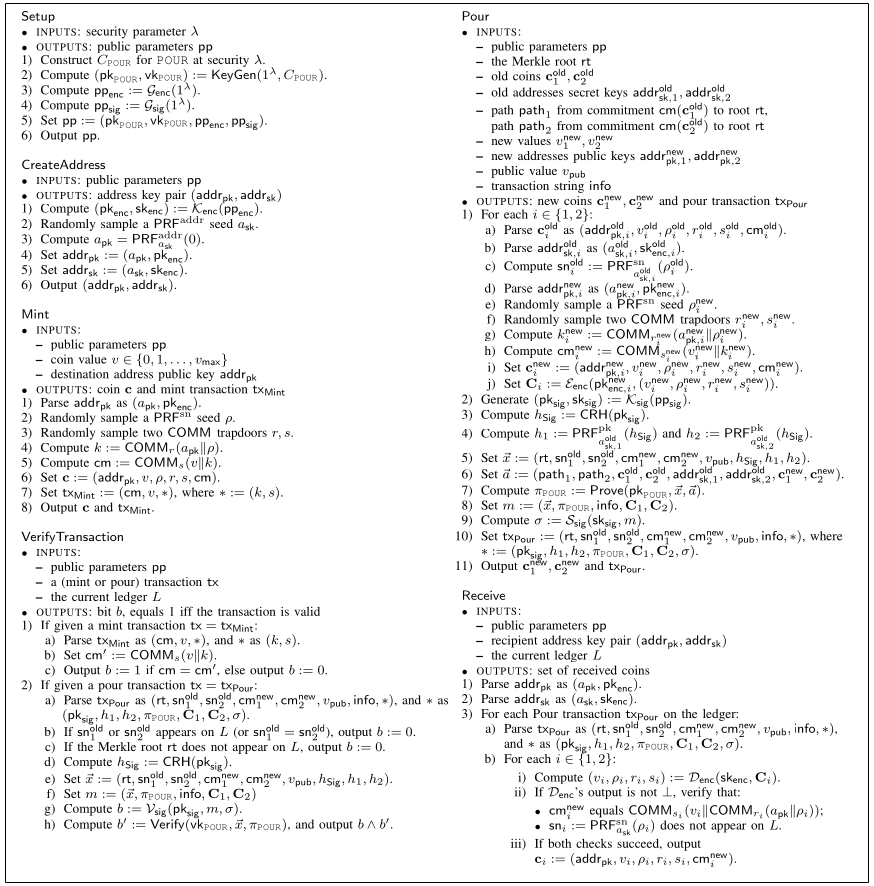
\includegraphics[width=\textwidth]{zerocash-zksnark.png}
\caption{The various operations performed in Zerocash. \cite{bensasson:zerocash}} \label{fig:zerocash}
\centering
\end{figure}

In case of a reorg, blocks and their transactions are no longer part of the active blockchain.
Provided that the spender is informed of his transaction's invalidation, he may decide to entirely recreate the transaction, including the zk-SNARK.
However, depending on the following conditions, it might only be necessary to modify some elements of $\vec{x}$ and $\vec{a}$ or none at all:

\begin{enumerate}
        \item \textit{\text{rt} references a state of the blockchain that both active and stale blockchain have in common.}
                if not, change rt, path1, path2
        \item \textit{$\text{c}_1^\text{old}$ and $\text{c}_2^\text{old}$ were in a block that is in the active blockchain.}
                There must have been a preceding block % TODO: blocks build chain, if preceding transaction also stale then recursive repeat, otherwise adapt this block. depeexnding on whther all blocks in chain belong to one user
 % todo: need to look at high-level like this and at zk-snark level internally in the circuit.
\ende{enumerate}

\section{Sprout}

Sprout uses zk-SNARKs from \cite{bensasson:zksnark}. They are implemented using a fork of the libsnark library \cite{zcash:libsnark}.

\begin{figure}[t]
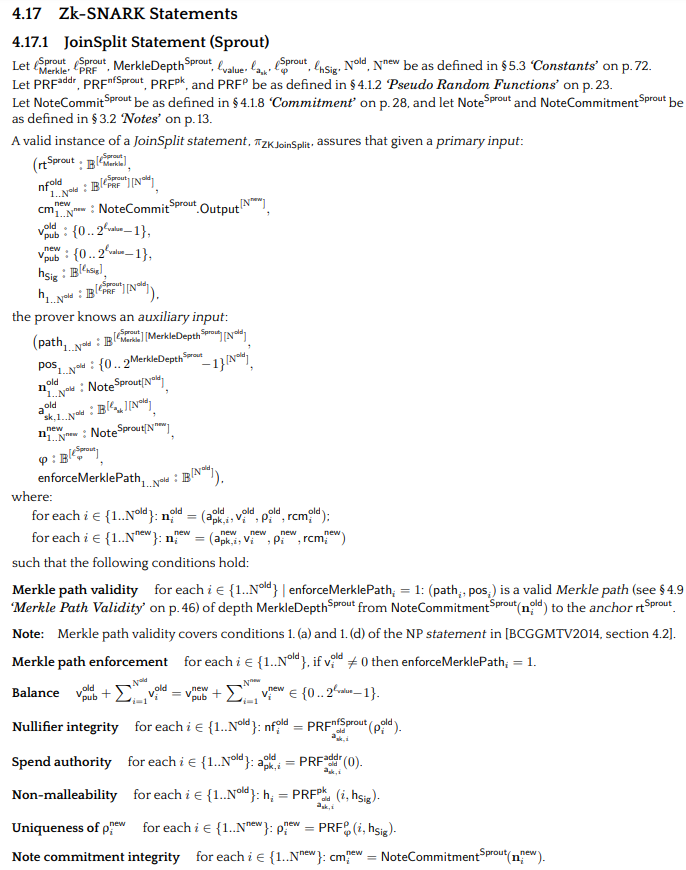
\includegraphics[width=\textwidth]{joinsplit-zksnark.png}
\caption{The zk-SNARK used for a JoinSplit description in the Sprout network update. \cite{hopwood:zcash}}
\centering
\end{figure}

\section{Sapling}

Sapling uses zk-SNARKs from \cite{groth:zksnark}. They are implemented using a Rust crate called bellman \cite{zcash:bellman}.

\begin{figure}[t]
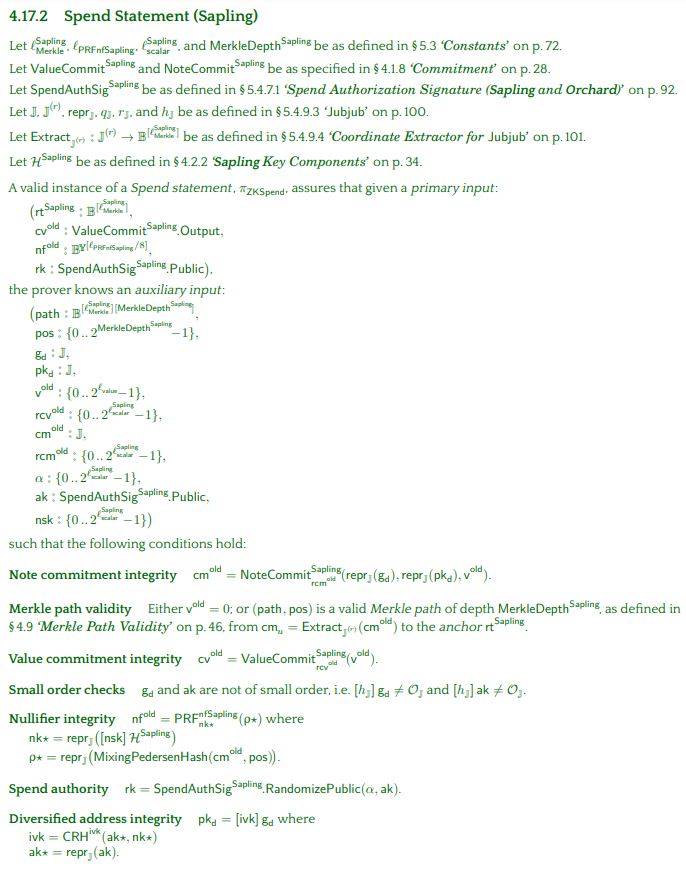
\includegraphics[width=\textwidth]{spend-zksnark.png}
\caption{The zk-SNARK used for a Spend description in the Sapling network update. \cite{hopwood:zcash}}
\centering
\end{figure}

\begin{figure}[t]
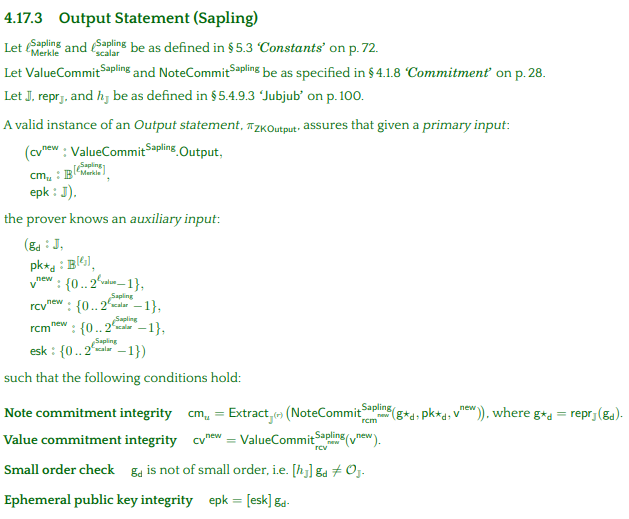
\includegraphics[width=\textwidth]{output-zksnark.png}
\caption{The zk-SNARK used for an Output description in the Sapling network update. \cite{hopwood:zcash}}
\centering
\end{figure}

\section{Orchard}

Orchard uses zk-SNARKs from \cite{zcash:halo2}.

\bibliographystyle{plain}
\bibliography{proofs}

\end{document}
